\chapter{Исследовательская часть}

В данном разделе будут приведены примеры работы программы и предоставлена информация о технических характеристиках устройства.

\section{Технические характеристики}

Ниже представлены характеристики компьютера, на котором проводились замеры времени работы реализации алгоритмов:

\begin{itemize}
	\item операционная система Windows 10 Домашняя 21H2;
	\item оперативная память 12 Гб;
	\item процессор Intel(R) Core(TM) i7-9750H CPU @ 2.6 ГГц.
\end{itemize}

\clearpage

\section{Демонстрация работы программы}

На рисунках \ref{img:example} -- \ref{img:example2} приведены примеры работы программы как показан в таблице \ref{tbl:tests}.

\begin{figure}[h]
	\begin{center}
		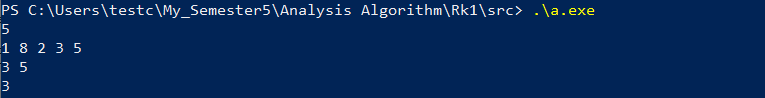
\includegraphics[scale=0.7]{img/example.png}
	\end{center}
	\captionsetup{justification=centering}
	\caption{Пример работы данного алгоритма при успешно поиске}
	\label{img:example}
\end{figure}


\begin{figure}[h]
	\begin{center}
		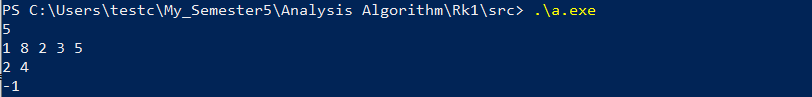
\includegraphics[scale=0.7]{img/example1.png}
	\end{center}
	\captionsetup{justification=centering}
	\caption{Пример работы данного алгоритма при неудачном поиске}
	\label{img:example1}
\end{figure}
\clearpage

\begin{figure}[h]
	\begin{center}
		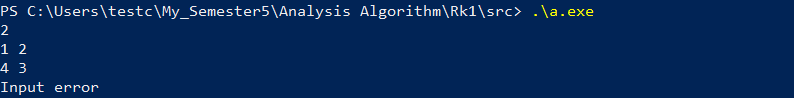
\includegraphics[scale=0.6]{img/example2.png}
	\end{center}
	\captionsetup{justification=centering}
	\caption{Пример работы данного алгоритма при неправильном вводе}
	\label{img:example2}
\end{figure}


\section{Вывод}
В данном разделе были приведены примеры работы программы.